\documentclass[crop, tikz]{standalone}


\begin{document}
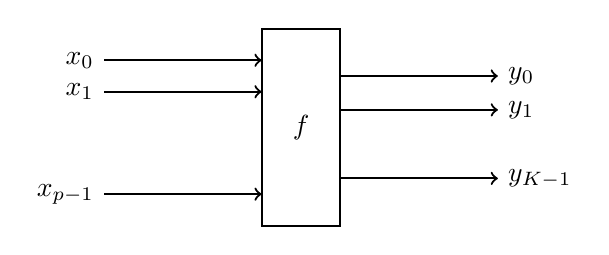
\begin{tikzpicture}
    \draw[thick] (2,0) rectangle (3, 2.5);
    \draw[thick, ->] (0,0.4) node[anchor=east] {$x_{p-1}$} -- (2,0.4);
    \draw[thick, ->] (0,1.7) node[anchor=east] {$x_1$} -- (2,1.7);
    \draw[thick, ->] (0,2.1) node[anchor=east] {$x_0$} -- (2,2.1);

    \draw[thick, ->] (3,{0.6}) -- (5,{0.6}) node[anchor=west] {$y_{K-1}$};
    \draw[thick, ->] (3,{1.9 - 0.43}) -- (5,{1.9 - 0.43}) node[anchor=west] {$y_1$};
    \draw[thick, ->] (3,{1.9}) -- (5,{1.9}) node[anchor=west] {$y_0$};

    \draw (2.5, 1.25) node {$f$};
\end{tikzpicture}

\end{document}
